\documentclass[10pt]{report}

\usepackage{amsmath}
\usepackage{mathptmx}
\usepackage{amssymb}
\usepackage{amsfonts}
\usepackage[utf8]{inputenc}
\linespread{1.2}
\usepackage{fancyhdr}
\usepackage{graphicx} % Required for inserting images
\usepackage[colorlinks,citecolor=blue]{hyperref}
\usepackage{tikz}
\usepackage{natbib}


\usepackage[a4paper,left=2.50cm, right=2.50cm, top=2.50cm, bottom=2.50cm]{geometry}

\author{Yiyang Zhang}

\title{Paper Reading Summary}
\author{Yiyang Zhang}


\begin{document}
\setlength{\parindent}{0pt}
\maketitle
\setcounter{tocdepth}{2}
\setcounter{secnumdepth}{4}

\tableofcontents
\newpage

\chapter{Option Market}



\chapter{Macro-Finance}
\section{Monetary Policy Shock}
\subsection{Monetary policy surprises and interest rates: Evidence from the Fed funds futures market (2001)}

\subsubsection{Contribution}

The main contribution of this paper by \citet{Kuttner2001MonetaryPS} is to provide empirical evidence on the differential response of bill, note, and bond yields to monetary policy actions using data from the Fed funds futures market. The paper distinguishes between anticipated and unanticipated policy actions, showing that while anticipated changes in the target rate have a minimal impact on interest rates, unanticipated changes significantly affect them. Additionally, the findings offer insights into the expectations hypothesis of the term structure of interest rates, explaining its lack of empirical support at the short end of the yield curve due to the limited effect of surprise target rate changes on expectations of future actions.

\subsubsection{Data}




\subsubsection{Methodology}



\subsubsection{Results}







\subsection{High-Frequency Identification of Monetary Non-Neutrality: The Information Effect (2018)}

\subsubsection{Contribution}
The main contribution of this paper by \citet{Nakamura2018HighFrequencyIO} is

\subsubsection{Data}




\subsubsection{Methodology}



\subsubsection{Results}






\chapter{Market MicroStructure}
\section{Trading Activities Identification from TAQ}
\subsection{Inferring Trade Direction from Intraday Data (1991)}
\subsubsection{Contribution}
This paper by \citet{LEE1991InferringTD} evaluates alternative methods for classifying individual trades as market buy or market sell orders using intraday trade and quote data. The authors document
two potential problems with quote-based methods of trade classification: quotes may be recorded ahead of trades that triggered them, and trades inside the spread are not readily classifiable. These problems are analyzed in the context of the interaction between exchange floor agents. The authors then propose and test relatively simple procedures for improving trade classifications.


\subsubsection{Data}

The dataset used for this paper are TAQ Trade and Quote dataset. 



\subsubsection{Methodology}
The specialist/market maker serves as both an auctioneer and a dealer. As an auctioneer, they match market orders with limit or standing orders, while as a dealer, they are ready to buy or sell on their own account. In this setting, trading generally takes place only when a market buy or sell order arrives. Since intraday data doesn't specify whether a trade was initiated by a market buy or sell order, this must be inferred from the data.

\paragraph{Price Only Method}

\begin{itemize}
    \item Tick Test
    \item Reverse Tick Test
\end{itemize}


\subsubsection{Results}



\subsubsection{Summary}






















\subsection{Caught on tape: Institutional trading, stock returns,
and earnings announcements (2009)}
\subsubsection{Contribution}


















\subsection{Tracking Retail Investor Activity (2021)}




\section{Trading Behavior Model}
\subsection{Option Volume and Stock Prices: Evidence on Where Informed Traders Trade (1998)}
\subsubsection{Contribution}
The main contribution of this paper by \citet{Easley1998OptionVA}











\clearpage
\section{Stock Price Information}




\subsection{Stock price clustering on option
expiration dates (2005)}

\subsubsection{Contribution}

The main contribution of this paper by \citet{XIAOYANNI2005StockPC} is that the authors presents striking evidence that option trading changes the prices of underlying stocks.
In particular, we show that \textbf{on expiration dates the closing prices of stocks with listed options cluster at option strike prices} (\textit{This is called Pinning Effect in the later literature}). On each expiration date, the returns of optionable stocks are altered by an average of at least 16.5 basis points, which translates into aggregate market capitalization shifts on the order of \$9 billion. The authors also provided evidence that hedge rebalancing by option market makers andstock price manipulation by firm proprietary traders contribute to the clustering.

\subsubsection{Data}
The datasets used for this paper is shown in the following:
\begin{itemize}
    \item Ivy DB dataset in OptionMetrics, range from January 4, 1996 through September 13, 2002.
    \item CBOE OpenClose Volume Summary Dataset, which contains trading volume data are broken down into eightcategories defined by four types of volume and two types of investors. Range from year 1996 to 2001.
\end{itemize}




\subsubsection{Methodology}
Here are the main methods the author used in the paper.
\begin{itemize}
    \item z-statistics method to check the distribution differences of pinning between different types of stocks within 21 days period (-10 to +10) around the option expiration date.
    \item \textbf{Pinning Definition: optionable stocks that have a daily closing price within \$0.125 of a strike price (of one of its own options) is defined as pinning.} For nonoptonal stocks, the pinning is defined as whether it concentrated around pirce at a integer multiplies \$5 (based on the building of equity option rules at that time).
    \item Absolut Differnce Distance Distribution Check: 
    \begin{itemize}
        \item Price Level: Price difference (adjacant interval with \$0.125 distance) between closing price and nearest strike price for expiration Friday and non-expiration Friday. 
        \item Return Level: Return difference (adjacant interval with 50 bps) for optional stocks between expiration Friday and non-expiration Friday. 
    \end{itemize}
    \item Lower Bound on the average deviation in the absolute returns of optionable stocks on expiration dates.
    $$
\text {Define } \hat{a}_i \equiv\left|\hat{r}_i\right| \text { and } a_i \equiv\left|r_i\right| \text {. Then }
\mathrm{E}\left|\hat{r}_i-r_i\right| \geqslant\left|\mathrm{E}\left(\hat{a}_i\right)-\mathrm{E}\left(a_i\right)\right|
$$
\begin{itemize}
    \item $\hat{r}_i$ denote the return on the stock in the $i$th optionable stock expiration date pair on expiration Friday, and $r_i$ denote what the return would have been in the absence of the expiration day effect (the unaltered stock return). 
    \item $\mathrm{E}\left|\hat{r}_i-r\right|$, measures the average effect on returns.
\end{itemize}
To apply this for different return difference intervals, the formula can be rewrite as 
$$
\left|\mathrm{E}\left(\hat{a}_i\right)-\mathrm{E}\left(a_i\right)\right| \approx \mid \sum_{b=1}^B[\hat{p}(b)-p(b)] a(b)
$$
\begin{itemize}
    \item $b=1, \ldots, B$ indexes $B$ absolute return intervals, $a(b)$ is the absolute return of interval $b$.
    \item $\hat{p}(b)-p(b)$ is the difference in the probability that an optionable stock's absolute return will fall in interval $b$ on expiration and nonexpiration Fridays.
\end{itemize}
\item Logistic Regression: The authors used a fixed-effects logistic regression model with a dependent variable that is set to one when the underlying stock price closes within \$0.125 of an option strike price, and zero
otherwise. And the authors built following independent variable to measure different mechanism.
\begin{itemize}
    \item \textbf{Market maker net purchased open interest}: Pinning pressure from the hedge rebalancing activities of likely delta hedgers.
    \item \textbf{New delta hedging}: measures pinning pressure from the delta hedging of changes in option positions
$$
\text { New delta hedging }\equiv \operatorname{sign}\left(S_{\text {Thur }}-K\right) \times\left(\text { DeltaAdjChgOI }{ }_{\text {Call }}^{M M}+\text { DeltaAdjChgOI } I_{\text {Put }}^{M M}\right)
$$ 
\begin{itemize}
    \item $\operatorname{sign}\left(S_{\text {Thur }}-K\right)$ takes the values $+1,0$, and -1 when the Thursday closing stock price is, respectively, greater than, equal to, or less than the nearest strike price
    \item DeltaAdjChgOI $I_{\text {Call/Put }}^{M M}$ is the delta-adjusted Thursday-to-Friday change in net market maker open interest aggregated across all calls/puts on the underlying stock
\end{itemize}
    \item \textbf{Covered call and protective put unwinding}: measures the unwinding by nondelta hedgers of positions that combine options and the underlying stock.
    $$
\text { CC\&PPunwinding }\\
 \equiv I\left(S_{\text {Thur }}-K\right) \times\left[\text { OTMPurchasedOI} _{\text {Put}}^{\text {Firm}}+\right.\text {Public} \left.+\text { OTMWrittenOI}_{\text {Call }}^{\text {Firm}+ \text {Public }}\right]
$$
\begin{itemize}
    \item $I\left(S_{\text {Thur }}-K\right)=1$ if the Thursday closing stock price is greater than the strike price nearest the Thursday closing stock price, and $I\left(S_{\text {Thur }}-K\right)=0$ otherwise. 
    \item OTMPurchasedOI$_{\text {Put }}^{\mathrm{Firm}+\text { Public }}$ is the purchased open interest of expiring OTM puts at the close on Thursday by firm proprietary traders and public customers.
    \item OTMWrittenOI$_{\text {Call }}^{\text {Firm }}+$ Public is the written open interest of expiring OTM calls at the close on Thursday by firm proprietary traders and public customers.
\end{itemize}
    \item The (absolute) distance between the Thursday closing stock price and the strike price nearest the Friday closing stock price.
\end{itemize}
\end{itemize}




\subsubsection{Results}
\begin{enumerate}
\item Pinning Facts Examination
\begin{itemize}
    \item Optionable stocks are more likely to close at or near strike prices on expiration dates.
    \begin{figure}[!h]
        \centering
        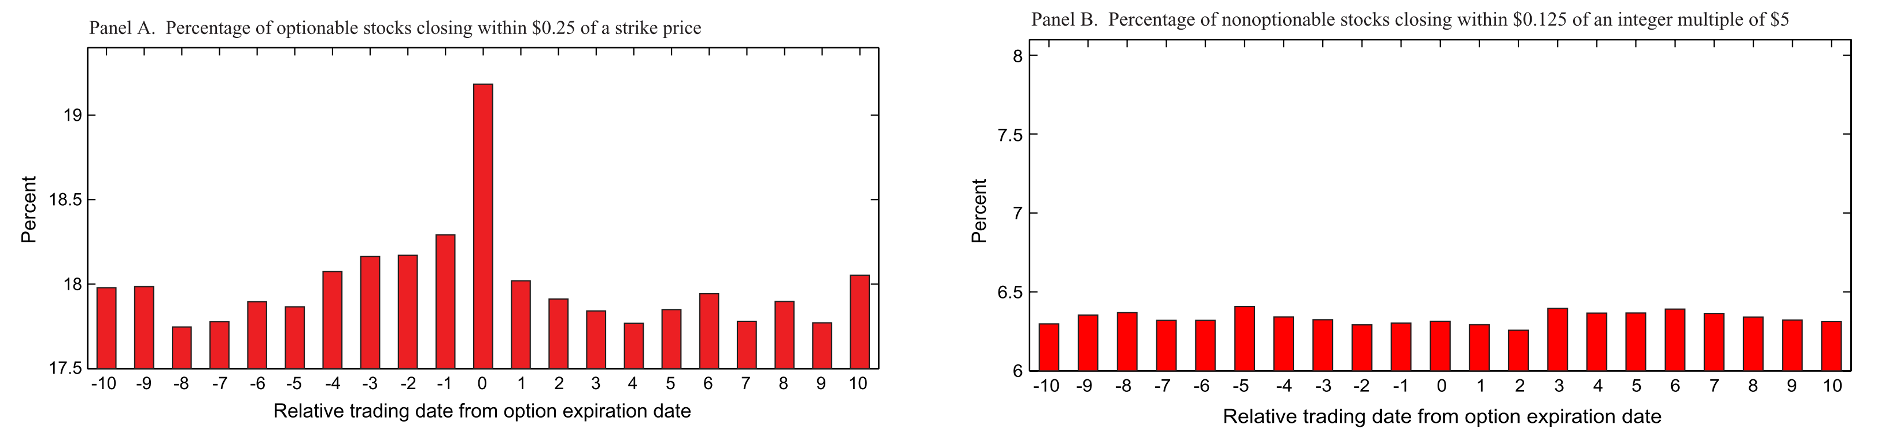
\includegraphics[width=1\linewidth]{p3.png}
        \caption{Difference between Optional stock and Nonoptional Stock}
    \end{figure}
    \begin{itemize}
        \item There is no expiration date clustering for the universe of nonoptionable stocks.
        \item The expiration date clustering appears when nonoptionable stocks become optionable anddisappears when optionable stocks become nonoptionable.
    \end{itemize}
    \item On expiration Fridays, more optionable stock prices close near a strike price and fewer close from \$0.50 to \$1.00 away from the nearest strike price. And on expiration Fridays optionable stocks are more likely to experience returns that are small in absolute value andless likely to experience returns that are large in absolute value. \textbf{This suggest that this pinning effect is from the stock price is prevented from leaving the neighborhood of the strike rather than cases in which Thursday stock prices distant from the strike are pushed to the strike.}
    \begin{figure}[!h]

                \centering
        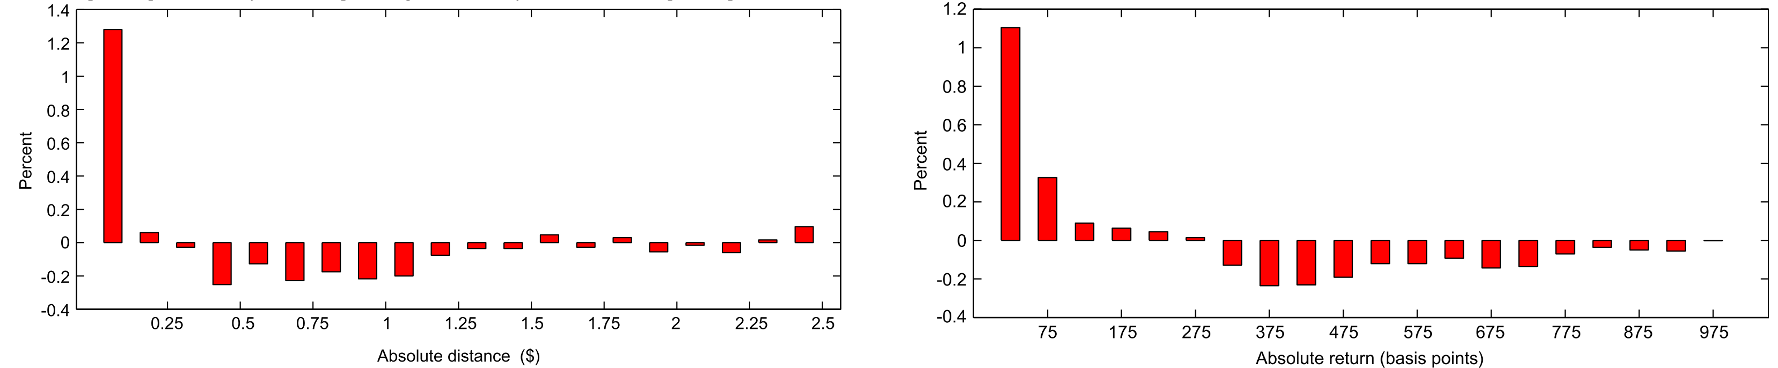
\includegraphics[width=1\linewidth]{p4.png}
        \caption{Distribution of Price Difference and Return Difference}
    \end{figure}
    \item The 16.57 bps lower bound on $\mathrm{E}\left|\hat{r}_i-r_i\right|$ implies that across optionable stocks the average expiration date alteration in absolute return is at least 16.57 bps.
\end{itemize}
\item Mechanism for Pinning: 
\begin{figure}[!h]
    \centering
    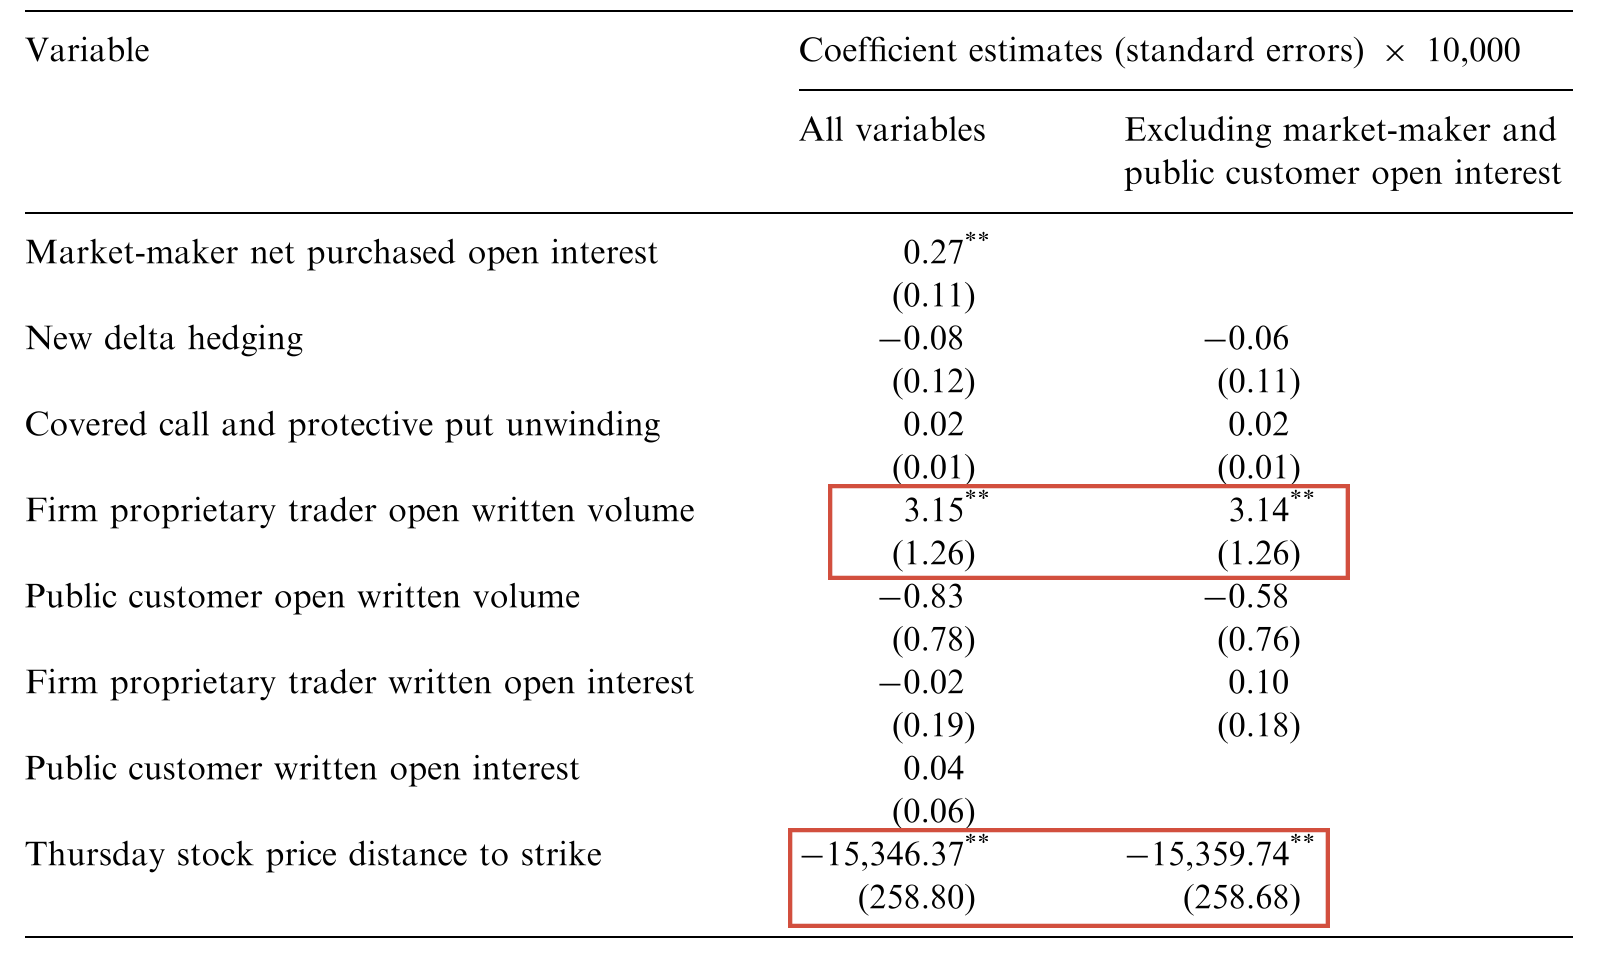
\includegraphics[width=0.75\linewidth]{p5.png}
    \caption{Mechanism Testing for Pinning}
\end{figure}
\begin{itemize}
    \item It is more likely that the stock price closes on or near an option strike price on the expiration Friday when the distance between the Thursday closing stock price and the strike price is smaller.
    \item The coefficient on market-maker net purchased open interest is positive and significant. This support hedge rebalancing.
    \begin{itemize}
        \item When delta hedgers have net purchased positions in the expiring options of an underlying stock with a particular strike price, hedge rebalancing will push the stock price toward the strike price and thereby tend to produce clustering.
        \item When delta hedgers have net written option positions, on the other hand, hedge rebalancing will push the stock price away from the strike price and thereby tend to produce declustering
    \end{itemize}
    \item There is no evidence that delta hedging of
changes in option positions or unwinding of combined stock and option positions by
nondelta hedgers contributes to the clustering.
\end{itemize}

\end{enumerate}




\subsubsection{Summary}

The conclusion of the study suggests that there is evidence of stock price clustering on option expiration dates, indicating the possibility of manipulation by option traders. The manipulation is more likely to be carried out by option writers with net written positions, as they have incentives to manipulate the stock price to prevent options from becoming in-the-money. On the other hand, option buyers with net purchased positions do not have the same incentives to manipulate the stock price. The study also acknowledges that there are costs and risks associated with manipulation, but the potential benefits may outweigh them for traders with larger option positions. Overall, the findings support the idea that option traders may manipulate underlying stock prices at expiration dates.




\clearpage
\subsection{Pinning in the S\&P 500 futures (2012)}

\subsubsection{Contribution}
The main contribution of this paper by \citet{Golez2012PinningIT} is that they shown \textbf{the Standard \& Poor’s (S\&P) 500 futures are pulled toward the at-the-money
strike price on days when serial options on the S\&P 500 futures expire (pinning) and are
pushed away from the cost-of-carry adjusted at-the-money strike price right before the
expiration of options on the S\&P 500 index (anti-cross-pinning).} And these effects are driven by
the \textbf{interplay of market makers’ rebalancing of delta hedges due to the time decay of those
hedges as well as in response to reselling (and early exercise) of in-the-money options by
individual investors.} The associated shift in notional futures value is at least \$115 million per
expiration day.

\subsubsection{Data}
Here is the data type and source summary.
\begin{itemize}
    \item Daily and Intraday data for S\&P 500 future: Chicago Mercantile Exchange (CME), range from April 21, 1982 to December 31, 2009.
    \item Daily SP options on S\&P 500 futures: Chicago Mercantile Exchange (CME), range from January 28, 1983 to December 31, 2009.
    \item Daily data for SPX options on the S\&P 500 index: Market Data Express, range from January 2, 1990 to December 31, 2009.
    \item SPX OpenClose data from CBOE Market Data Express, range from January 2, 1990 to December 31, 2009. \textbf{For the number of open contracts bought by individual customers}.
    \item SOQ / SET for special AM exercise-settlement values from Market Data Express. Quarterly SOQ values run from June 1991 to December 2009, and serial SOQ values run from November 1992 to November 2009.
\end{itemize}

\subsubsection{Methodology}

\begin{itemize}
    \item \textbf{Pinning Effect: on option expiration days, stock prices tend to finish more frequently near a strike price.} (The fact that pinning occurs only on expiration dates is different from clustering, which is the tendency of prices to be quoted on particular round values. Such clustering is independent of a day being an expiration day or not).
    \item Test of Pinning Effect: Logistic Regression with Fixed Effect, and authors focused on the ten days before and after the expiration date. And the model is defined as following:
    $$
    \operatorname{Pr}\left(\text { Pinn\_sym }_t=1\right)=\frac{1}{\left.1+e^{\left[-\left(\alpha+\beta \text { Dumm }_t\right)\right.}\right]}
    $$
    \item The pinning effect binaray variable $\text { Pinn\_sym }_t$ is defined as
    $$
\text { Pinn\_sym }_t= \begin{cases}1, & \text { if }\left|F u t_t-K_t^{A T M}\right| \leq 0.375 \\ 0, & \text { otherwise. }\end{cases}
$$
which is one if the
futures price at settlement is within \$0.375 below or
above the at-the-money strike price and zero otherwise.
    \item Authors define $\text{Dumm}_t$ as one for expiration days and zero otherwise. In this way above logistic regression tests if pinning on expiration days is significantly higher than on nonexpiration days. The variable $\text{Dumm}_t$ can also be changed to different variables to examine the machinsiam.
    \item The pinning dummy can also be split to two different cases. The futures price is pushed below its fair value or the futures price is above its fair value. 
    $$
\begin{aligned}
&\begin{aligned}
& \text { Pinn\_above }_t=\left\{\begin{array}{lr}
\text { Pinn\_sym }_t=1 \text { and } & \text { Fut }_t \leq \text { Fut }_t{ }^*   \\
0, & \text { otherwise }
\end{array}\right.
\end{aligned}\\
&\text { Pinn\_above }_t=\left\{\begin{array}{lr}
\text { Pinn\_sym }_t=1 \text { and } & \text { Fut }_t \leq \text { Fut }_t{ }^*  \\
0, & \text { otherwise }
\end{array}\right.
\end{aligned}
$$
\end{itemize}



\subsubsection{Results}

\begin{enumerate}
    \item Pinning Effect:
    \begin{figure}[!h]
        \centering
        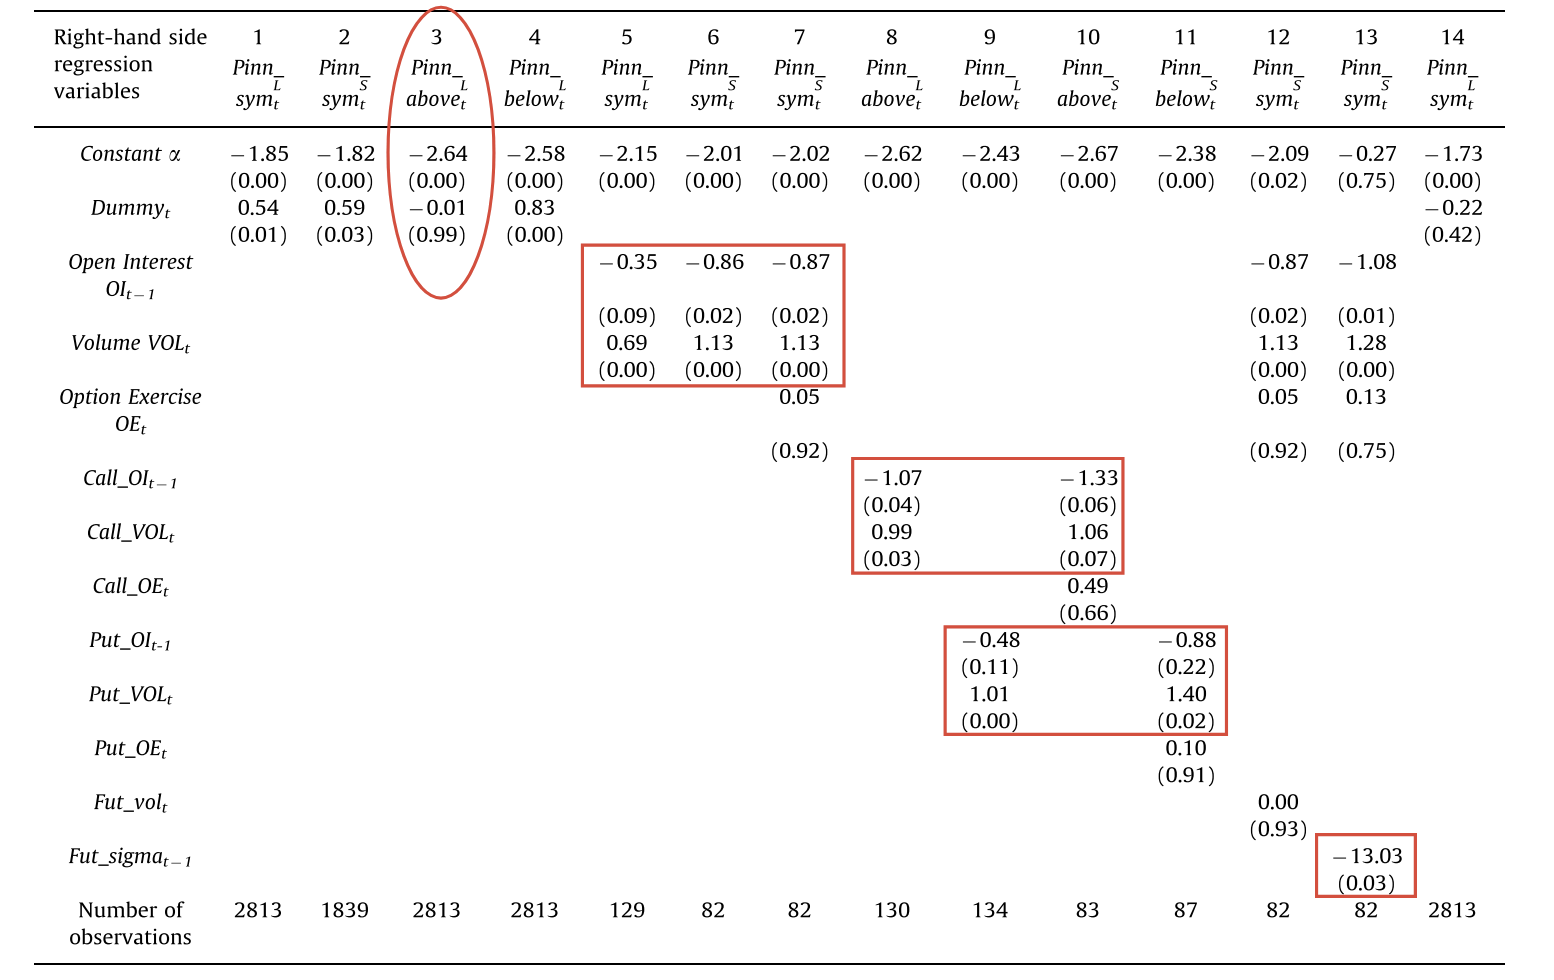
\includegraphics[width=1\linewidth]{p1.png}
        \caption{Key Result for Pinning Effect}
        \label{p1}
    \end{figure}
    \begin{itemize}
        \item Pinning does exist in the first-to-maturity future due to serial SP options. And at-the-money open interest decreases pinning while the at-the-money option volume (both call and put) increases pinning.
        \begin{itemize}
            \item \citet{Avellaneda2003AMM} argue that the time decay of delta hedges of long option positions leads to pinning. Alas, given that index option market makers typically hold short (i.e., written) option positions, their mechanism leads to anti-pinning in the index futures.
            \item The larger the at-the-money open interest on expiration Friday, the larger are the sold option positions that market makers need to hedge. Thus, the higher the open interest, the weaker the pinning and the stronger the anti-pinning effect.
            \item On expiration Friday, at-the-money option volume largely reflects the closing of expiring positions. Higher volume tends to reduce open interest, diminishing market makers’ hedging needs and increasing the likelihood of pinning behavior.
        \end{itemize}
        \item Underlying future's volatility decrease pinning.
        \begin{itemize}
            \item Futures volatility makes delta hedging of market makers more difficult and is, therefore, negatively related to pinning.
        \end{itemize}
        \item Early option exercise for both put and call at-the-money option and underlying future volume are not related to pinning.
        \begin{itemize}
            \item There is no significant evidence for early exercise.
            \item Given the associated risks — such as price risk, detection risk, and pin risk—the authors argue that market makers and proprietary traders are likely deterred from engaging in such activities, rendering manipulation an unlikely explanation for residual pinning.
        \end{itemize}
        \item There is no pinning for second-to-maturity future and S\&P 500 index due to serial SP options.
        \begin{itemize}
            \item The authors express skepticism that market makers’ hedging activities could exert enough influence to move the entire basket of 500 stocks.
        \end{itemize}
   \end{itemize}
    \item Cross Pinning Effect: This means for SPY option market, the market maker may not hedging the underlying asset itself (500 bucket stocks), but hedging on the future market instead. In this case, the SPX market could cross-pin onto the future market.
    \begin{figure}[!h]
        \centering
        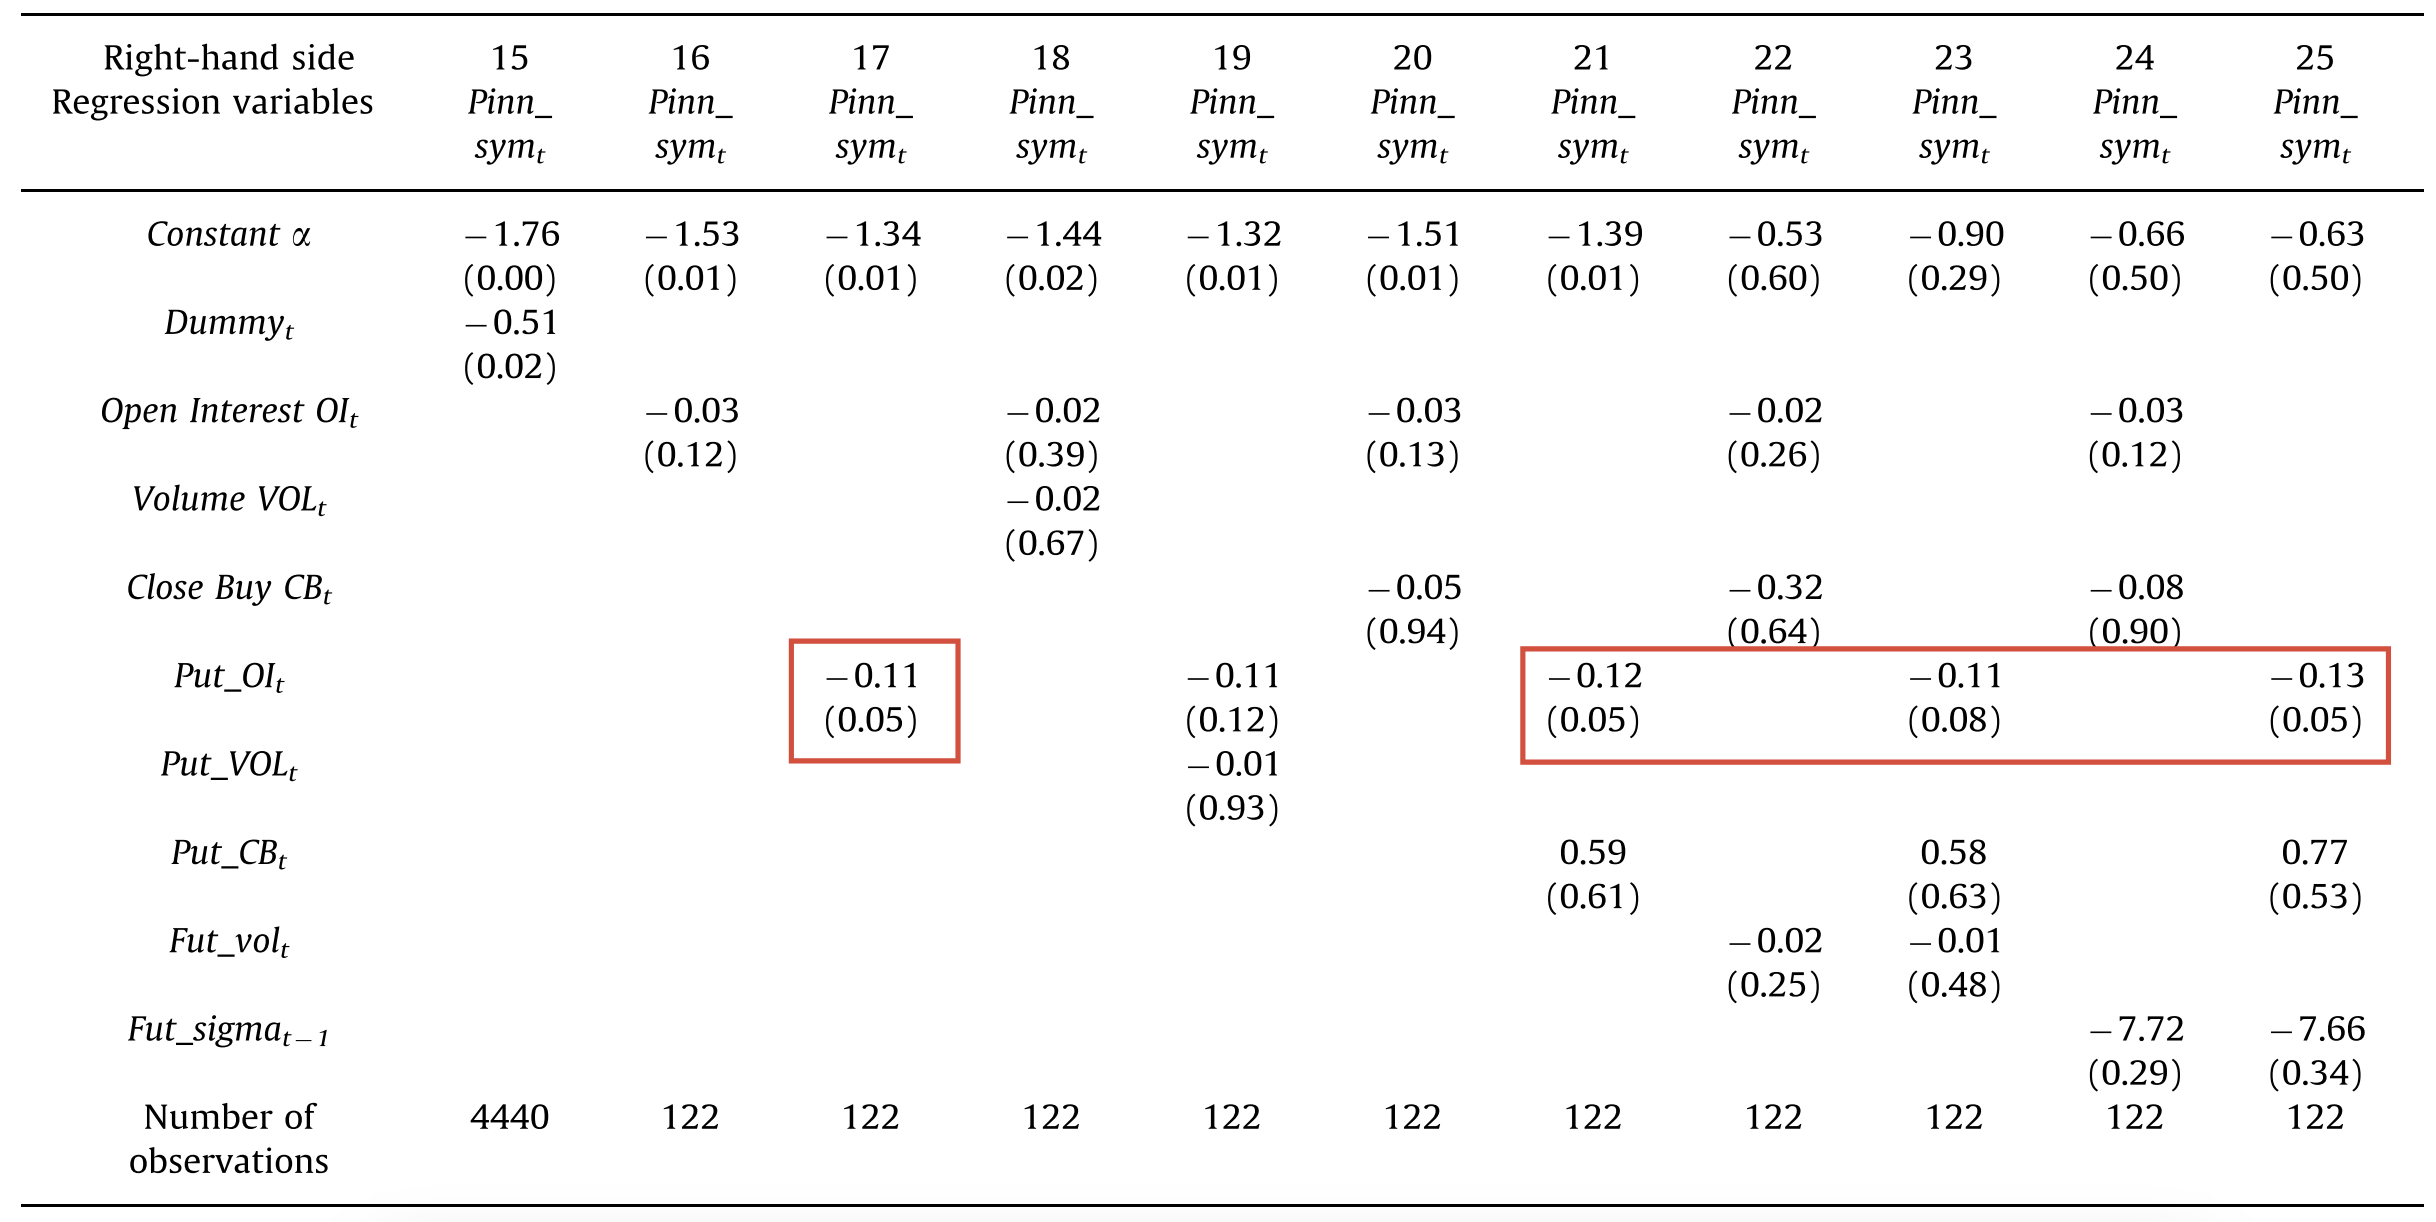
\includegraphics[width=1\linewidth]{p2.png}
        \caption{Key Result for Cross-Pinning Effect}
        \label{p2}
    \end{figure}
    \begin{itemize}
    \item Cross Pinning Effect does exist.
    \item At-the-money open interest decrease the pinning effect, this align with the mechanism of \citet{Avellaneda2003AMM}, and the put option rather than the all options is significant is reasonable because the market maker position in put is much higher than call.
\end{itemize}
\end{enumerate}
\subsubsection{Summary}

The study concludes that SP options cause pinning in the S\&P 500 futures market, where the futures prices tend to gravitate toward strike prices on option expiration days. This phenomenon is unexpected, as financial theory generally suggests that all potential closing prices of the underlying asset are equally probable. The study finds that the mechanisms driving pinning in index futures differ significantly from those in individual stocks. While stock pinning is influenced by market makers' delta hedging, this doesn't fully explain index futures pinning. Instead, the study suggests two contributing factors: the physical settlement of serial SP options leading to hedging pressure and SPX options being hedged via S\&P 500 futures, causing anti-cross-pinning. The study also notes significant, temporary movements of futures values toward the nearest strike price on expiration days, which could raise concerns for regulators and exchanges. Overall, the research sheds light on the distinct mechanisms of pinning in the S\&P 500 futures market compared to stocks.



\clearpage
\subsection{Does option trading convey stock price information? (2014)}
\subsubsection{Contribution}

The main contribution of this paper by \citet{Hu2014DoesOT} is that, the authors shown that after executing option orders, options market makers turn to the stock market to hedge away the underlying stock exposure. As a result, the stock exposure imbalance in option transactions translates into an imbalance in stock transactions. T\textbf{his paper decomposes the total stock order imbalance into an imbalance induced by option transactions and an imbalance independent of options.} The analysis shows that the o\textbf{ption-induced imbalance significantly predicts future stock returns in the cross section controlling for the past stock and options returns, but the imbalance independent of options has only a transitory price impact.} Further investigation suggests that options order flow contains important information about the underlying stock value.


\subsubsection{Data}

Here is the data type and source summary. All the data range from 2008 April to 2010 August.
\begin{itemize}
    \item Options Transaction Data: Trade Alert LCC. It provides all of the trade messages recorded by the Options Price Reporting Authority (OPRA). And it also provides classification for an option trade as buyer/seller-initiated if the transaction price is above (below) the most recent mid quote price (Common Stocks Only).
    \item Stock Transaction Data: TAQ Dataset. And the transaction direction is based on \citet{LEE1991InferringTD}, and opening and closing 15 minutes are excluded from the data for direction classification accuracy.
    \item Stock Price Information: CRSP.
    \item The number of analysts following is extracted from the Institutional Brokers0 Estimate System (I/B/E/S), and the institutional ownership data are from the Form 13-F filings in the Thomson Reuters database.
\end{itemize}

\subsubsection{Methodology}
\begin{itemize}
    \item Order Imbalance Definition:
    \begin{itemize}
        \item Option Order Imbalance (OOI): \citet{Holowczak2014AggregatingII} show that risk exposure to the underlying stock price (delta) is an important consideration when extracting the stock price information from option transactions.
        $$
        \text { OOI }_{i, t}=\frac{\sum_{j=1}^n 1_j \text { 100Dir }_{i, t, j} \cdot \text { delta }_{i, t, j} \cdot \text { size }_{i, t, j}}{\text { Num\_share\_outstanding }}
        $$
        For stock $i$ on day $t$, the numerator is the aggregate delta position of the active options traders who initiate the trades. And the scale by outstanding shares is used for removing the uninformed trade during the inactive trading period.
        \begin{itemize}
            \item $\operatorname{Dir}_{i, t, j}$ is a dummy variable equal to one (negative one) if the $j$ th option trade is initiated by the buyer (seller) according to certain trade signing algorithms. 
            \item The delta$_{i, t, j}$ is the option price's sensitivity to the underlying stock price.
            \item The size$_{i, t, j}$ denotes the trade size in option lots (one hundred shares of the underlying stock).
        \end{itemize}
        And OOI also measures the net delta hedging demand in the stock market.
        \item Stock Order Imbalance (SOI): The stock order imbalance (SOI) unrelated to the options market is the difference between the total order imbalance (TOI) in the stock market and the OOI.
        $$
\mathrm{SOI}_{i, t}=\mathrm{TOI}_{i, t}-\mathrm{OOI}_{i, t}=\frac{\sum_{j=1}^N \text { Dir }_{i, t, j} \cdot \text { size }_{i, t, j}}{\text { Num\_shares\_outstanding }_i}-\mathrm{OOI}_{i, t}
$$where $\mathrm{TOI}_{i, t}$ is in terms of the trading volume, and $\operatorname{Dir}_{i, t, j}$ and $\operatorname{size}_{i, t, j}$ are the direction dummy and the size of the $j$ th stock transaction of firm $i$ on day $t$, respectively.
    \end{itemize}
    \item Models Used for Testing is mainly Fama-MacBeth Regression
    \begin{itemize}
        \item Model to Test Return Predictability: $$
\operatorname{Ret}_{i, t}=\alpha+\sum_{k=1}^5 \beta_1^k \mathrm{SOI}_{i, t-k}+\sum_{k=1}^5 \beta_2^k \mathrm{OOI}_{i, t-k}+\theta X_{i, t-1}+\varepsilon_{i, t}
$$$X_{i, t-1}$ is a set of control variables composed of the closing percentage bid-ask spread of the stock, the stock's turnover ratio as the total trading volume scaled by the number of shares outstanding, the log trading volumes in the two markets, and the stock returns and the equally weighted options returns from the past five days.

This model is also used for the test for level of information asymmetric, institutional ownership and market activity's impact on the predictive ability of OOI.
\begin{itemize}

        \item Information Asymmetric: Based on probability of informed trading (PIN) / the number of stock analysts following the firm / the bid–ask spread in the stock market / the adverse-selection component of the bid–ask spread / and the firm size, sort the data and divided into three groups using threshold of 30\% and 70\%.
        \item Institutional Ownership and Market Activity also sorted and divided into three groups similarly.
    \end{itemize}
    \item Model to Test Option Leverage:
$$\operatorname{Ret}_{i,t}=\alpha+\sum_{k=1}^5\left(\beta_1^k \text {OTM\_OOI}_{i,t-k}+\beta_2^k \text {ATM\_OOI}_{i,t-k}\right. \left.+\beta_3^k \text {ITM\_OOI}_{i,t-k}\right)+\sum_{k=1}^5 \beta_4^k \text {SOI}_{i,t-k}+\theta X_{i,t-1}+\varepsilon_{i,t}$$
\begin{itemize}
    \item At-the-money: $0.375 < |\text{delta}| < 0.625$
    \item In-the-money: $|\text{delta}| > 0.625$
    \item Out-of-the-money: $|\text{delta}| < 0.375$
\end{itemize}
    \end{itemize}
\end{itemize}






\subsubsection{Results}
\begin{enumerate}
    \item Return Predictability:
    \begin{itemize}
        \item Both of the stock and options trading volumes significantly predict returns, but in opposite directions.
        \item The SOI does not positively predict future returns. The reversal effect on day $t+2$ indicates that the price impact of the SOI is more likely to come from transitory price pressure rather than from an information flow.
        \item The OOI positively predicts the stock returns on the next day, and the predictability does not reverse in longer horizons.
        \item These findings thereby provide unambiguous evidence that the options order flow contains a significant amount of private information about the
        underlying stock's price movement. The results are shown in Table \ref{p6}.
        \item For the equally weighted quintile portfolios are formed based on each order imbalance variable. The excess return is significant at the 1\% level after controlling for the Fama and French risk factors and the momentum factor. The findings in this table show that the return predictability from the OOI is economically significant. The results are shown in Table \ref{p7}.
    \end{itemize}
    \begin{figure}[!h]
        \centering
        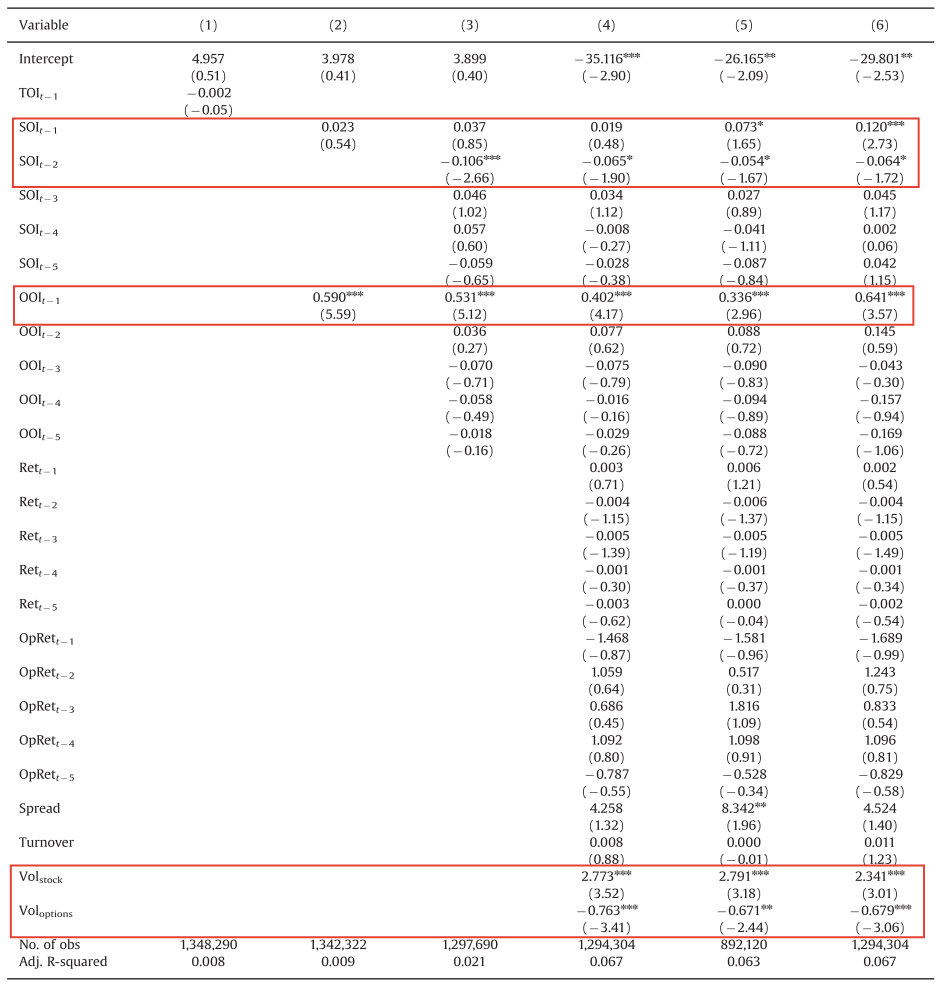
\includegraphics[width=1\linewidth]{p6.png}
        \caption{Daily Level Return Predictability Analysis}
        \label{p6}
    \end{figure}

    \begin{figure}[!h]
        \centering
        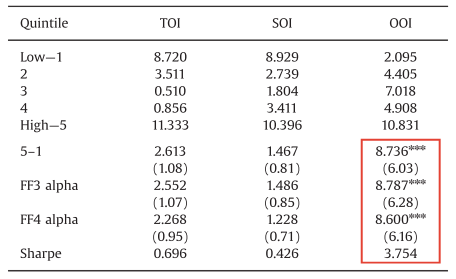
\includegraphics[width=0.5\linewidth]{p7.png}
        \caption{Daily Level Portfolio Analysis}
        \label{p7}
    \end{figure}
    \item Intraday Level Analysis
    \begin{itemize}
        \item The SOI positively predicts the next half-hour returns with a coefficient significant positive. However, the predictive relation becomes significantly negative in the following half-hour.
        \item The OOI positively predicts the next half-hour returns significantly but not significantly for the following half-hour.
        \item The high-frequency results confirm the previous findings at the daily frequency that the OOI has a permanent price impact and that the SOI generates only transitory price pressure as shown in Table \ref{p8}.
    \end{itemize}
    \begin{figure}[!h]
        \centering
        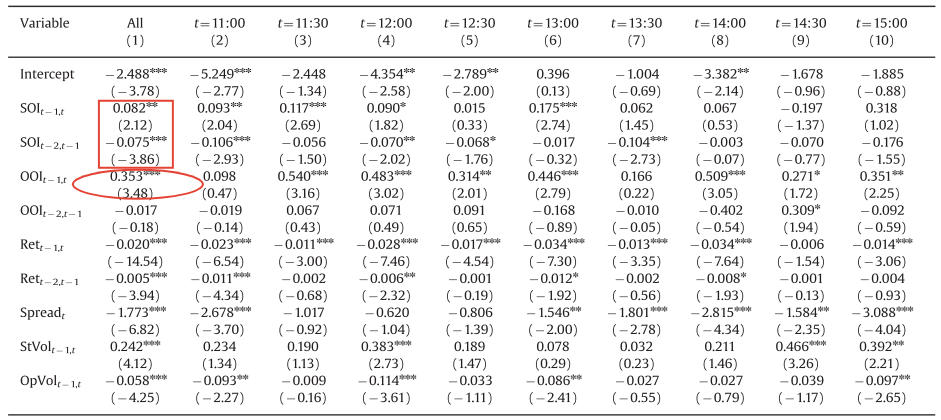
\includegraphics[width=1\linewidth]{p8.png}
        \caption{Intraday Level Return Prediction Analysis}
        \label{p8}
    \end{figure}
    \item There is no empirical support for option leverage, a possible explanation is that many institutional investors use the OTM options to gain volatility exposures, and the order imbalance does not contain much information about the underlying stock price. Another possibility is that the transaction costs associated with the OTM options are too high.
    \item Level of Information Asymmetry, Institutional Ownership, and Market Activity
    \begin{figure}[!h]
        \centering
        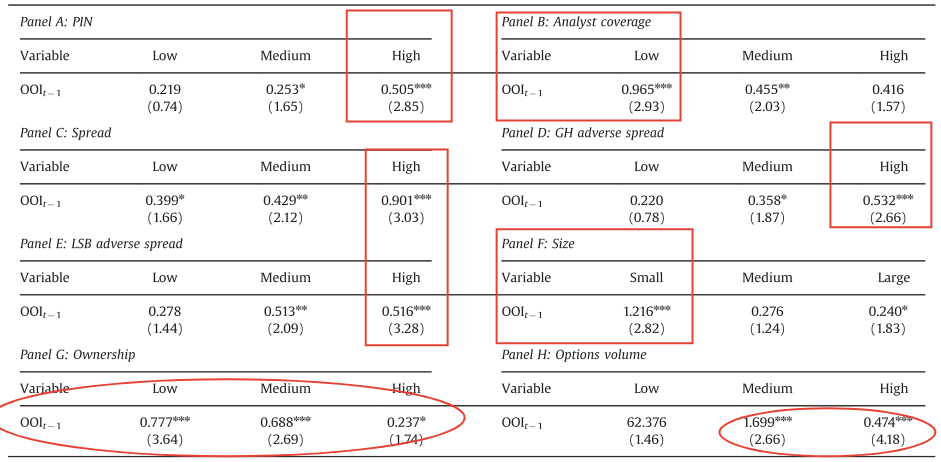
\includegraphics[width=1\linewidth]{p9.png}
    \end{figure}
    \begin{itemize}
        \item OOI has a stronger predictive powerfor returns when the firm has a higher level of information asymmetry.
        \item Higher Institutional Ownership reduce the short-sale constraint. The results suggest that short-sale constraints in the stock market increase the information content in the options order flow.
        \item OOI does not significantly predict the underlying returns when the options trading volume is low. The predictive ability of the OOI comes from the periods when the options market is active. 
    \end{itemize}
    \item Asymmetric Price Response
    \begin{figure}[!h]
        \centering
        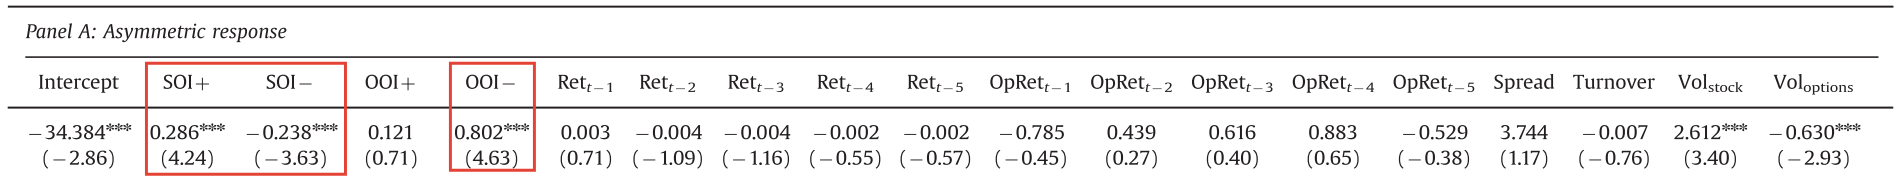
\includegraphics[width=1\linewidth]{p10.png}
    \end{figure}
    \begin{itemize}
        \item SOI is divided into  $\mathrm{SOI}_{i, t-1}^{+}=\max \left(\mathrm{SOI}_{i, t-1}, 0\right)$ and $\mathrm{SOI}_{i, t-1}=\min \left(\mathrm{SOI}_{i, t-1}, 0\right)$. OOI is also divided into $\mathrm{OOI}_{i, t-1}^{+}=\max \left(\mathrm{OOI}_{i, t-1}, 0\right)$ and $\mathrm{OOI}_{i, t-1}^{-}=\min \left(\mathrm{OOI}_{i, t-1}, 0\right)$.
        \item Both the positive and negative SOIs significantly predict stock returns, but the signs are inconsistent. This is why overall SOI does not exhibit an ability to predict stock returns.
        \item The predictive power of the OOI mainly comes
from the negative OOI, which support that
informed traders use options to get around the short-sale
constraints in the stock market when they acquire negative
information.
    \end{itemize}
    \item Event Study around Earning Announcement
    \begin{figure}[!h]
        \centering
        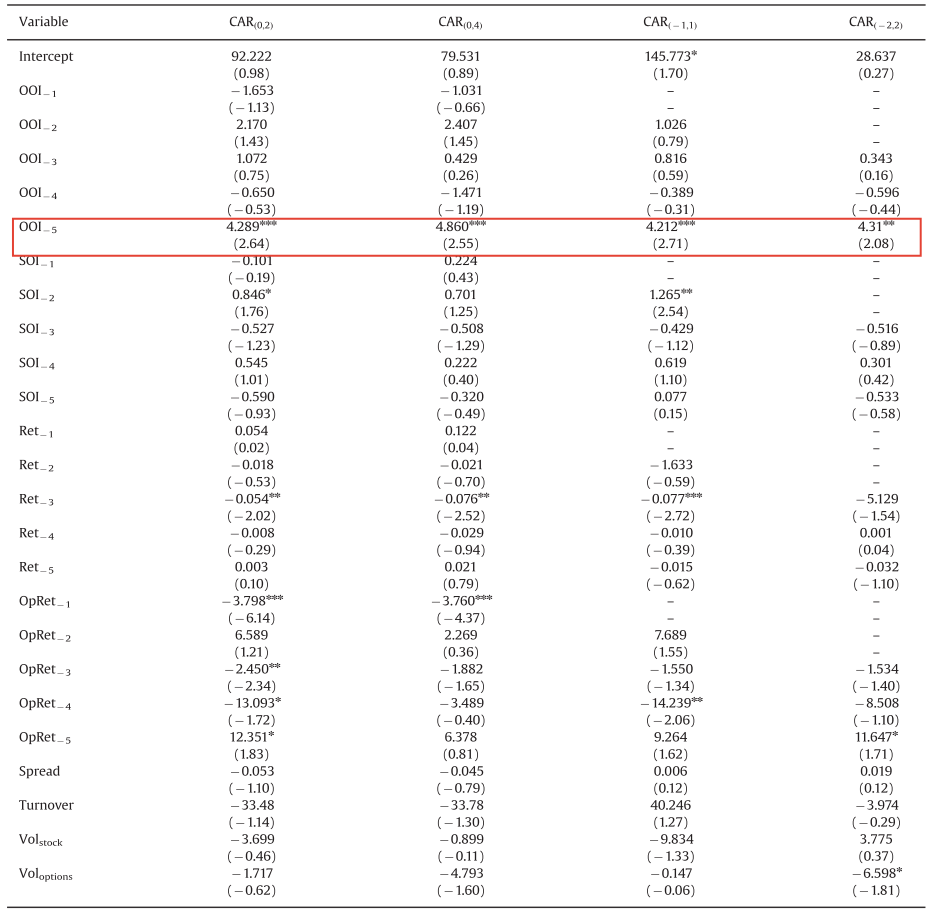
\includegraphics[width=0.95\linewidth]{p11.png}
    \end{figure}
    \begin{itemize}
        \item Risk Adjusted Return for firms is calculated based on \citet{Carhart1997OnPI}.
        \item The options market conveys information about corporate earnings five days before the announcement.
        \item High Earnings Surprise, Analysts's Dispersion, and low Analysis Coverage groups' significant result shows Informed trading is more active when the potential profit is high.
    \end{itemize}
    \begin{figure}[!h]
        \centering
        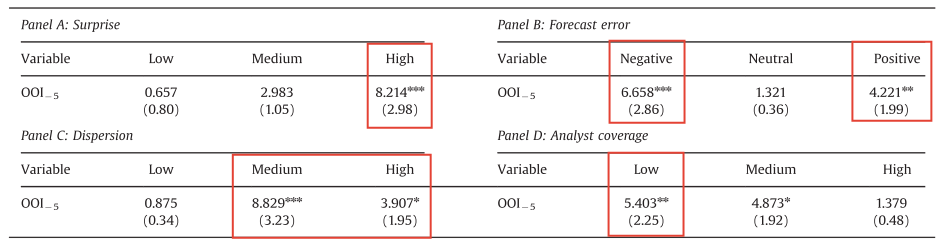
\includegraphics[width=1\linewidth]{p12.png}
    \end{figure}
\end{enumerate}










\subsubsection{Summary}

The paper concludes that options trading provides valuable insights into stock price movements, with options order imbalance (OOI) showing a significant positive impact on future stock returns. The analysis reveals that OOI from at-the-money (ATM) and in-the-money (ITM) options predicts future returns, while OOI from out-of-the-money (OTM) options does not. Additionally, OOI is found to have stronger predictive power for firms with higher levels of information asymmetry, although the effects of institutional ownership and market activity on OOI’s predictive ability are less definitive. These findings suggest that OOI can be a useful tool for investors to anticipate stock price movements and make more informed trading decisions. Also, the permanent price information in stock order flow is induced mostly by option transactions, which suggests that informed traders do use options as a trading tool.










\bibliography{reference.bib}
\bibliographystyle{jfe}




\end{document}
